\documentclass[25pt, a0paper, portrait, margin=0mm, innermargin=15mm,
  blockverticalspace=8mm, colspace=15mm, subcolspace=8mm]{tikzposter}

% ============================================
% ECSA 2026 Poster - A0 Portrait
% Style: University of Limerick official green
%   branding (Green / White / Grey), light grey
%   blocks, serif titles, sans body text
% ============================================

\usepackage[utf8]{inputenc}
\usepackage[T1]{fontenc}
\usepackage{lmodern}
\usepackage{amsmath,amssymb}
\usepackage{booktabs}
\usepackage{graphicx}
\usepackage{xcolor}
\usetikzlibrary{arrows.meta}

% ---------- Colour palette (University of Limerick official green branding) ----------
\definecolor{leroBlue}{HTML}{1B5E3C}      % UL institutional green (header band)
\definecolor{leroAccent}{HTML}{7AC142}     % bright UL accent green
\definecolor{leroGrey}{HTML}{F2F2F2}      % light block background
\definecolor{leroDark}{HTML}{1A1A1A}

\usetheme{Simple}

\colorlet{backgroundcolor}{white}
\colorlet{blocktitlebgcolor}{leroBlue}
\colorlet{blocktitlefgcolor}{white}
\colorlet{blockbodybgcolor}{leroGrey}
\colorlet{blockbodyfgcolor}{leroDark}
\colorlet{blockbodyborder}{leroBlue}
\colorlet{titlefgcolor}{white}
\colorlet{titlebgcolor}{leroBlue}

\usetitlestyle[titletotopverticalspace=0mm, titletoblockverticalspace=1cm]{Filled}
\useblockstyle[roundedcorners=4, linewidth=0pt, titleinnersep=0.6cm, bodyinnersep=1cm]{Basic}

\tikzposterlatexaffectionproofoff

% ============================================
% Institutional logos (UL, Maastricht, Lero, Horizon Globex)
% sourced from logos/ and converted/trimmed as needed.
% Logos are trimmed to their tight bounding box and scaled
% by height (not width) so every logo box is a uniform size
% with equal padding, regardless of the logo's native aspect ratio.
% NOTE: boxes are sized to their image content (not the full column
% width) so there is no extra left/right whitespace inside the box.
% ============================================
\setlength{\fboxsep}{0.12cm}
\title{\begin{minipage}{0.98\linewidth}
\begin{minipage}[c]{0.18\linewidth}
  \centering
  \fcolorbox{white}{white}{\parbox[c][2.1cm][c]{\linewidth}{\centering
\includegraphics[height=1.8cm]{logos/ul-trim.png}}}\\[3mm]
  \fcolorbox{white}{white}{\parbox[c][2.1cm][c]{\linewidth}{\centering
\includegraphics[height=1.8cm]{logos/maastricht-trim.png}}}
\end{minipage}\hfill
\begin{minipage}[c]{0.54\linewidth}
  \centering\color{white}\bfseries
  A Lock Free, Non-blocking, In Line Processing Architecture for\\
  High Throughput and Regulatory Compliant Blockchain Trading Applications
\end{minipage}\hfill
\begin{minipage}[c]{0.18\linewidth}
  \centering
  \fcolorbox{white}{white}{\parbox[c][2.1cm][c]{\linewidth}{\centering
\includegraphics[height=1.8cm]{logos/lero-trim.png}}}\\[3mm]
  \fcolorbox{white}{white}{\parbox[c][2.1cm][c]{\linewidth}{\centering
\includegraphics[height=1.8cm]{logos/horizon-trim.png}}}
\end{minipage}
\end{minipage}}
\author{\color{white}
  Andrew Le Gear$^{1}$ \quad
  Jim Buckley$^{1}$ \quad
  Tawny Whatmore$^{2}$ \quad
  Ashish Sai$^{3}$}
\institute{\color{white}\small
  $^{1}$CSIS Department, Lero, University of Limerick, Ireland \quad
  $^{2}$Horizon Globex Ireland, Ireland \quad
  $^{3}$Department of Advanced Computing Sciences, Maastricht University, Netherlands \\[2mm]
  \normalsize andrew.p.legear@ul.ie \quad | \quad ECSA 2026, Bolzano, Italy \quad | \quad Artifact: Zenodo DOI 10.5281/zenodo.21512313}

\begin{document}

\maketitle

\begin{columns}

% ============================================
% LEFT COLUMN
% ============================================
\column{0.33}

\block{Motivation}{
  \begin{itemize}
    \item Regulated decentralised finance (DeFi) requires trading systems that are simultaneously \textbf{high-throughput} and \textbf{regulatory compliant}.
    \item Off-chain compliance checks (KYC/AML, trade surveillance) and on-chain settlement pull system design in opposite directions.
    \item Existing blockchain trading architectures are not empirically benchmarked against production-grade throughput and latency targets.$^{[1]}$
    \item \textbf{Research question:} which architectural pattern maximises throughput while preserving compliance guarantees, under real blockchain constraints (nonce ordering, gas limits, block capacity)?
  \end{itemize}
}

\block{Approach}{
  \begin{itemize}
    \item Two-layer \textbf{hybrid architecture}: off-chain compliance / order layer decoupled from on-chain settlement layer.
    \item \textbf{Ablation study} of five progressively optimised architectural variants, deployed and measured on a live production trading system.
    \item Variants isolate the effect of: asynchronous submission, multi-threading, multi-wallet parallelism, and symbol-level sharding with lock-free coordination.
    \item Empirical measurement of throughput, latency (avg / P99), and block utilisation for each variant under identical load.
  \end{itemize}
}

\block{Two-Layer Hybrid}{
  \begin{center}
    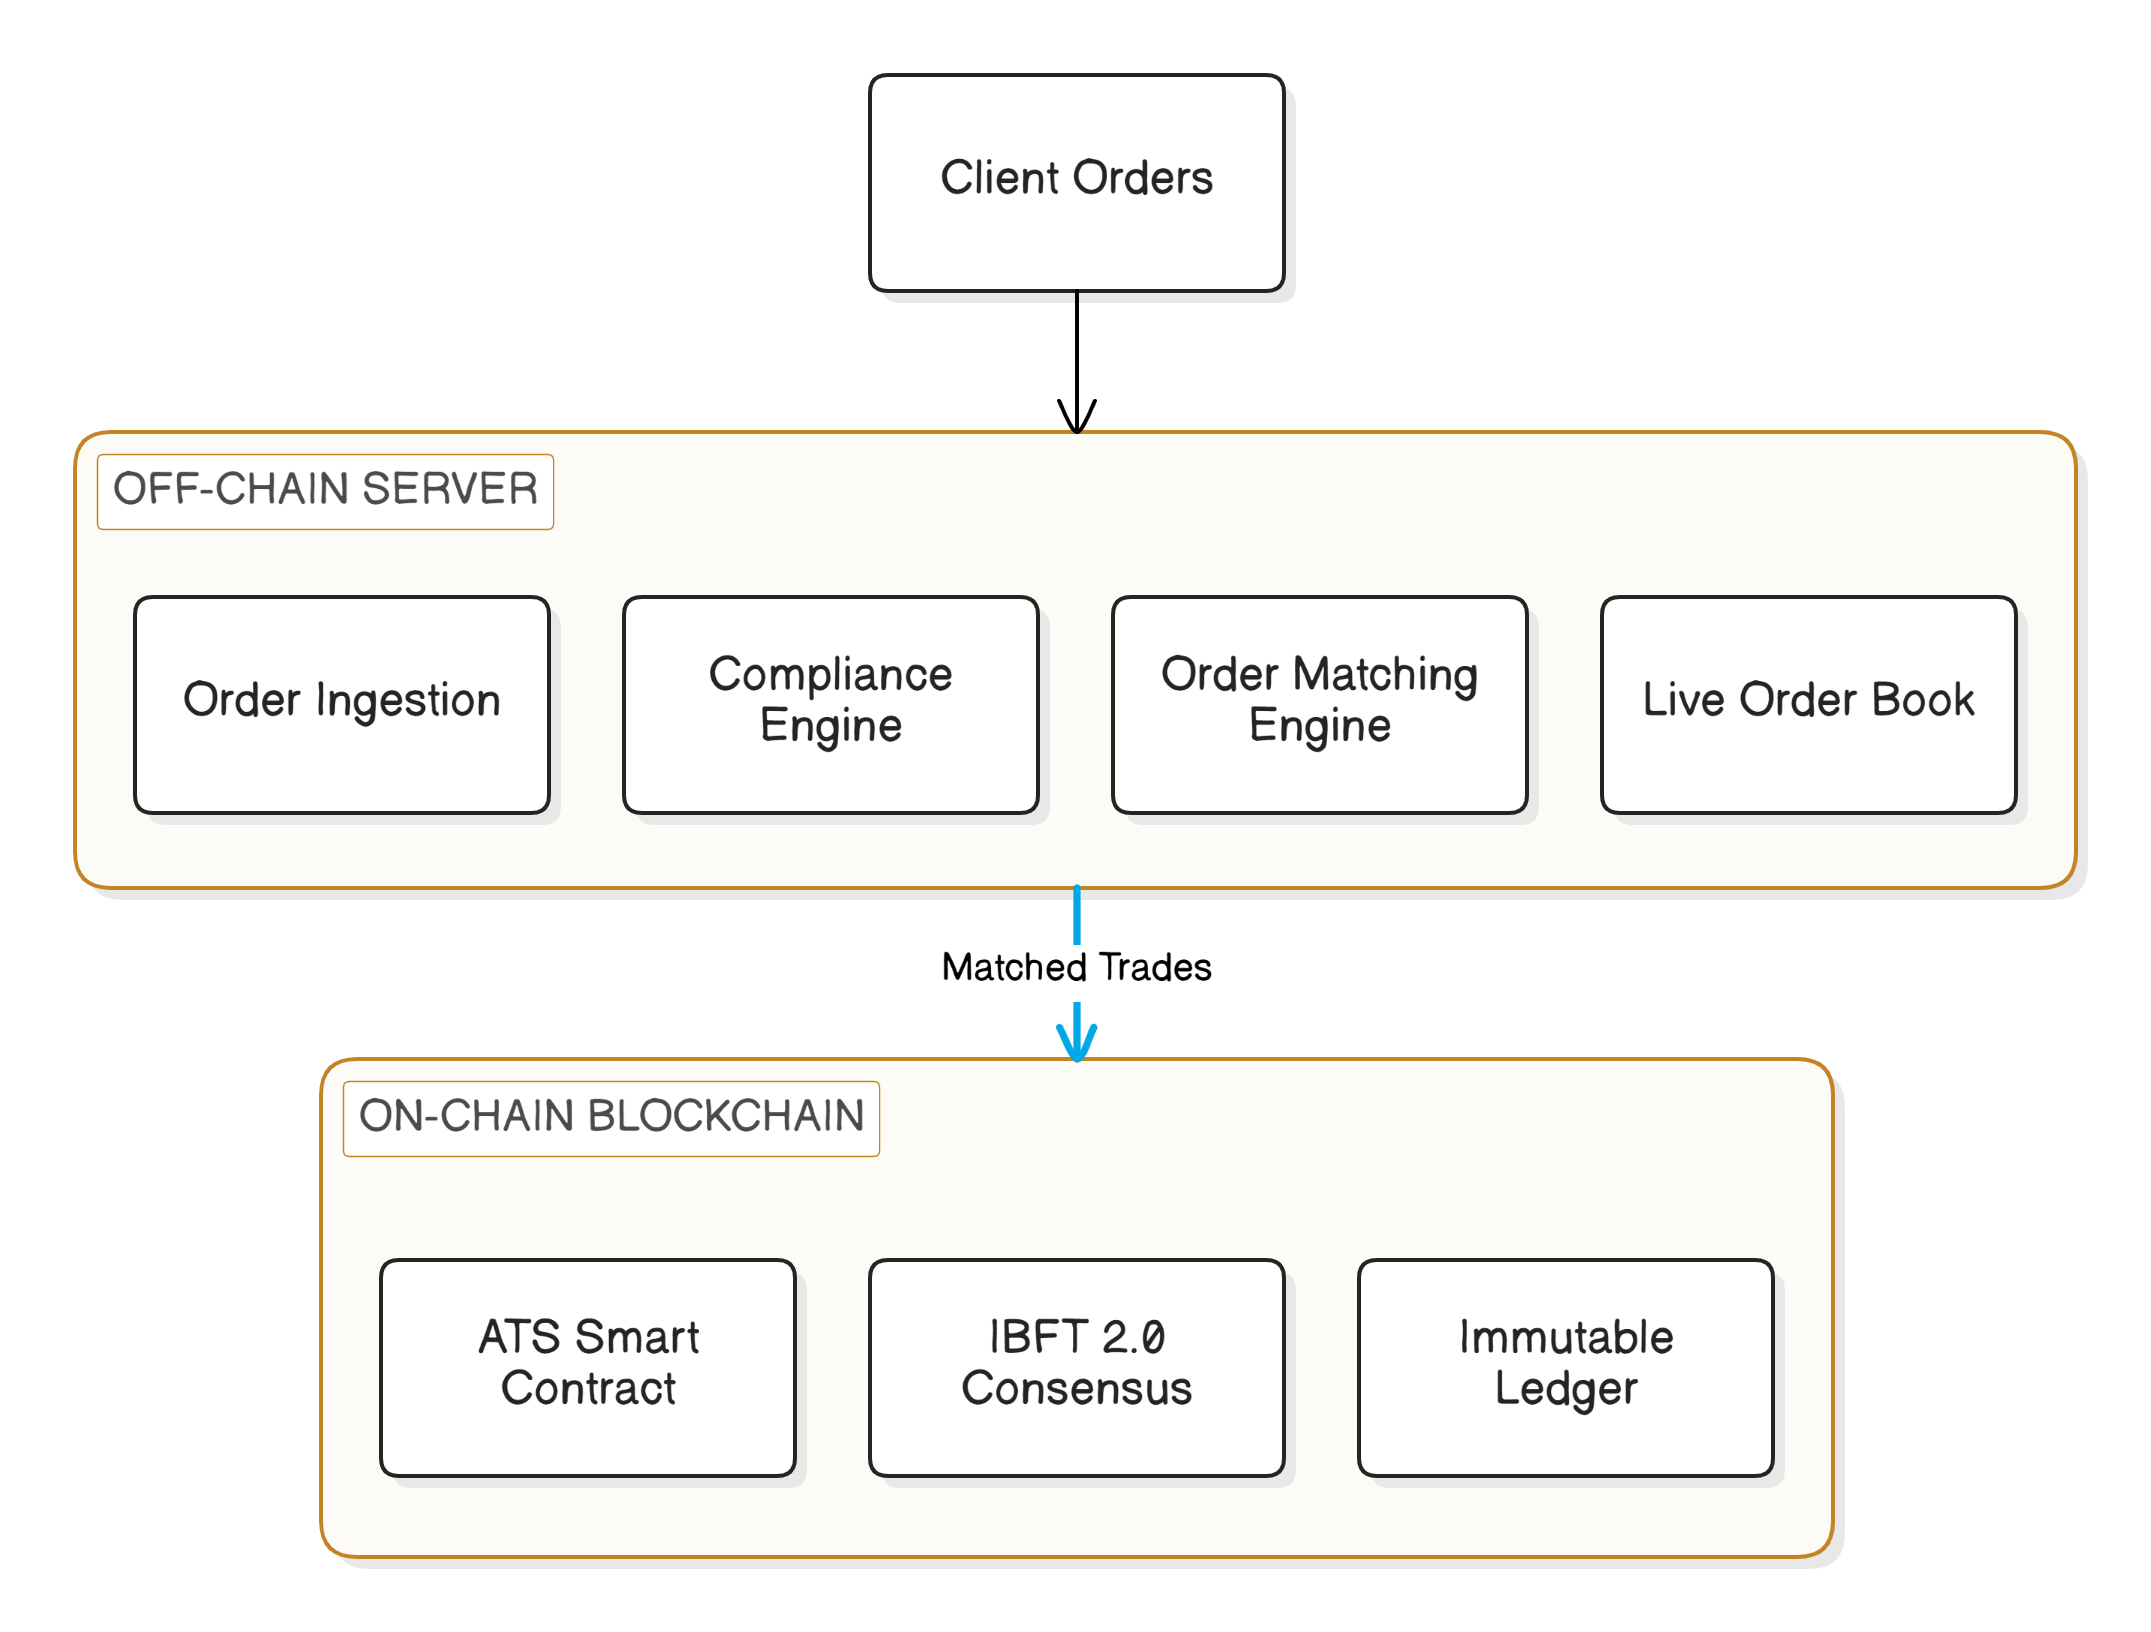
\includegraphics[width=0.77\linewidth]{images/two-layer-model.png}\\[0.1cm]
    \footnotesize\textbf{Fig.~1:} 2-layer hybrid architecture.
  \end{center}
  \vspace{0.15cm}
  Off-chain compliance, matching, and order-book components are decoupled from on-chain settlement, keeping regulatory logic mutable while the ledger stays immutable.

  \vspace{0.2cm}
  \textbf{Five architectural stages studied:}
  \begin{enumerate}
    \setlength\itemsep{0.05em}
    \item Sequential, blocking, single wallet
    \item Asynchronous, single wallet
    \item Multi-threaded, asynchronous, single wallet
    \item Unsynchronised multi-threaded, multi-wallet
    \item \textbf{Symbol-sharded, lock-free, multi-wallet (proposed)}
  \end{enumerate}
}

\block{Industry Profile}{
  \begin{itemize}
    \item \textbf{Horizon Globex Ireland DAC} is a fintech services company delivering blockchain-backed trading and exchange systems.
    \item Deployments include US automated trading systems and the \textbf{Upstream} platform in the Seychelles.
    \item Upstream supports \textbf{MERJ}, a tier-one regulated stock exchange.
  \end{itemize}
}

% ============================================
% MIDDLE COLUMN
% ============================================
\column{0.34}

\block{Key Findings}{
  \begin{itemize}
    \item \textbf{Nonce mechanism} limits naive parallelism to only a \textbf{36\% throughput gain} — Ethereum's strict per-account nonce ordering is a hard serialisation point.$^{[4]}$
    \item Circumventing nonce ordering with multiple wallets \textbf{without} careful coordination causes a \textbf{9$\times$ increase in latency} due to lock contention.
    \item Bottlenecks \textbf{migrate}: solving one on-chain constraint exposes a new server-side concurrency crisis.$^{[2]}$
    \item Our \textbf{lock-free, symbol-sharded} submission model (inspired by HFT architectures) removes contention entirely by partitioning work per trading symbol.$^{[3,6]}$
  \end{itemize}
}

\block{Performance Results}{
  \begin{center}
    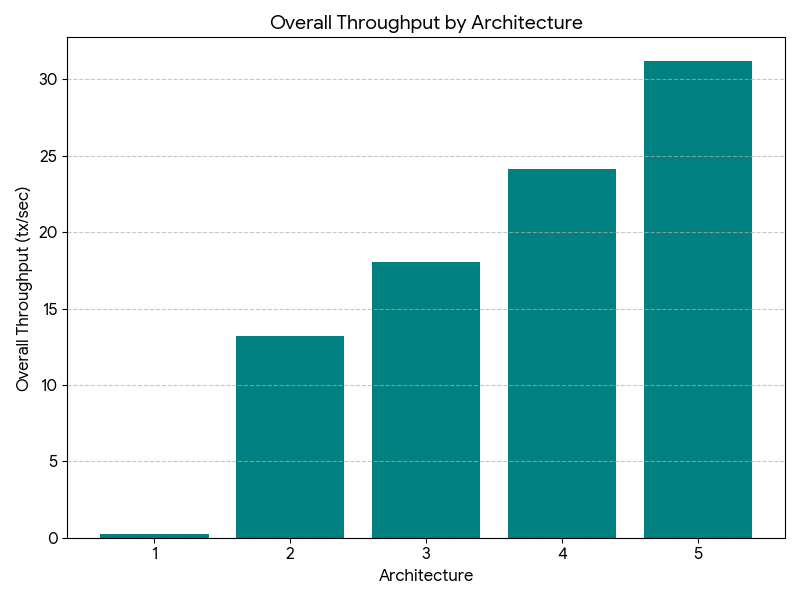
\includegraphics[width=0.86\linewidth]{images/stat1.png}\\[0.1cm]
    \footnotesize\textbf{Fig.~2:} Throughput across architectural stages.\\[0.4cm]
    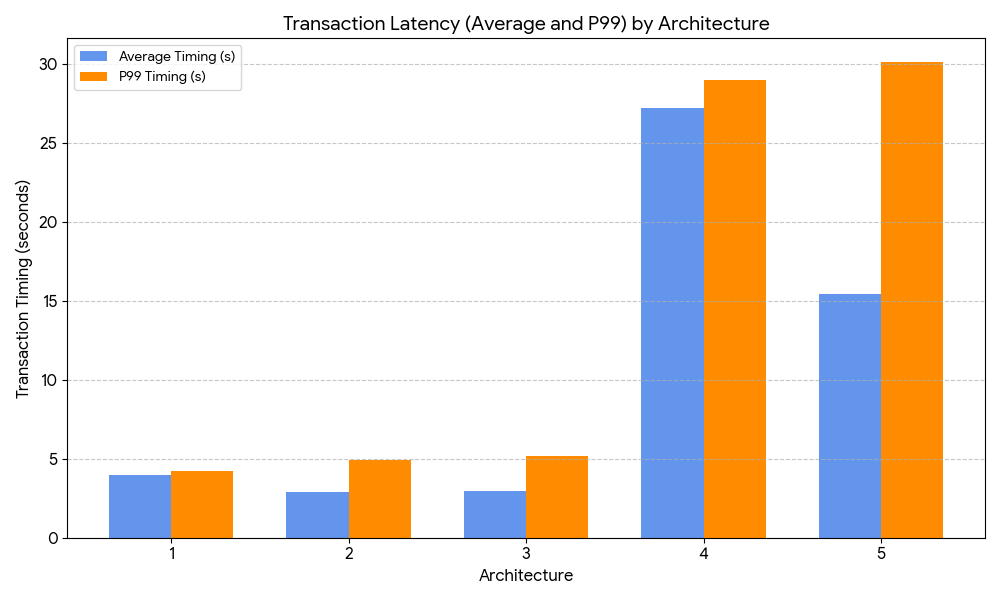
\includegraphics[width=0.47\linewidth]{images/stat2.png}\hfill
    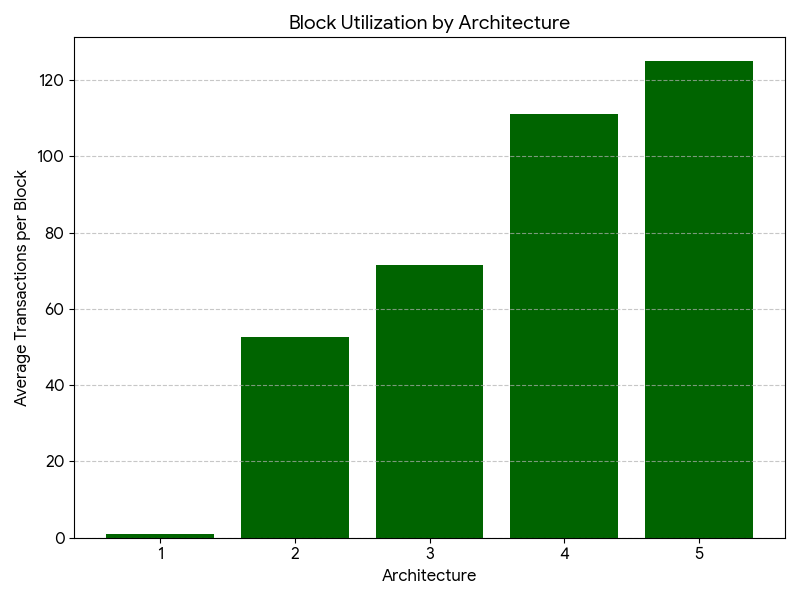
\includegraphics[width=0.47\linewidth]{images/stat3.png}\\[0.1cm]
    \footnotesize\textbf{Fig.~3:} Latency \hfill \textbf{Fig.~4:} Block utilisation\hspace{0.4cm}
  \end{center}
  \vspace{0.4cm}
  \begin{center}
    \Large\bfseries\color{leroBlue}
    2.8$\times$ improvement over conventional design\\
    125$\times$ gain over naive baseline\\
    44\% latency reduction at peak throughput
  \end{center}
}

\block{Why It Matters}{
  \begin{itemize}
    \item Demonstrates that \textbf{holistic co-design} of on-chain and off-chain components is essential --- optimising either layer in isolation is insufficient.
    \item Provides an empirically validated architecture pattern directly applicable to production regulated-DeFi trading systems.
    \item Highlights blockchain-specific constraints (nonce ordering, gas limits, block capacity) as first-class architectural drivers, not implementation details.
  \end{itemize}
}

\block{Production System}{
  \begin{itemize}
    \item \textbf{Upstream} is Horizon Globex's live platform, running \textbf{Architecture~5} (symbol-sharded, lock-free) in production.
    \item Off-chain server handles order ingestion, KYC/AML, and matching.
    \item Settlement via permissioned \textbf{IBFT~2.0} Ethereum and the \texttt{ATS.sol} contract.
  \end{itemize}
}

% ============================================
% RIGHT COLUMN
% ============================================
\column{0.33}

\block{Symbol-Sharded, Lock-Free Design}{
  \begin{center}
    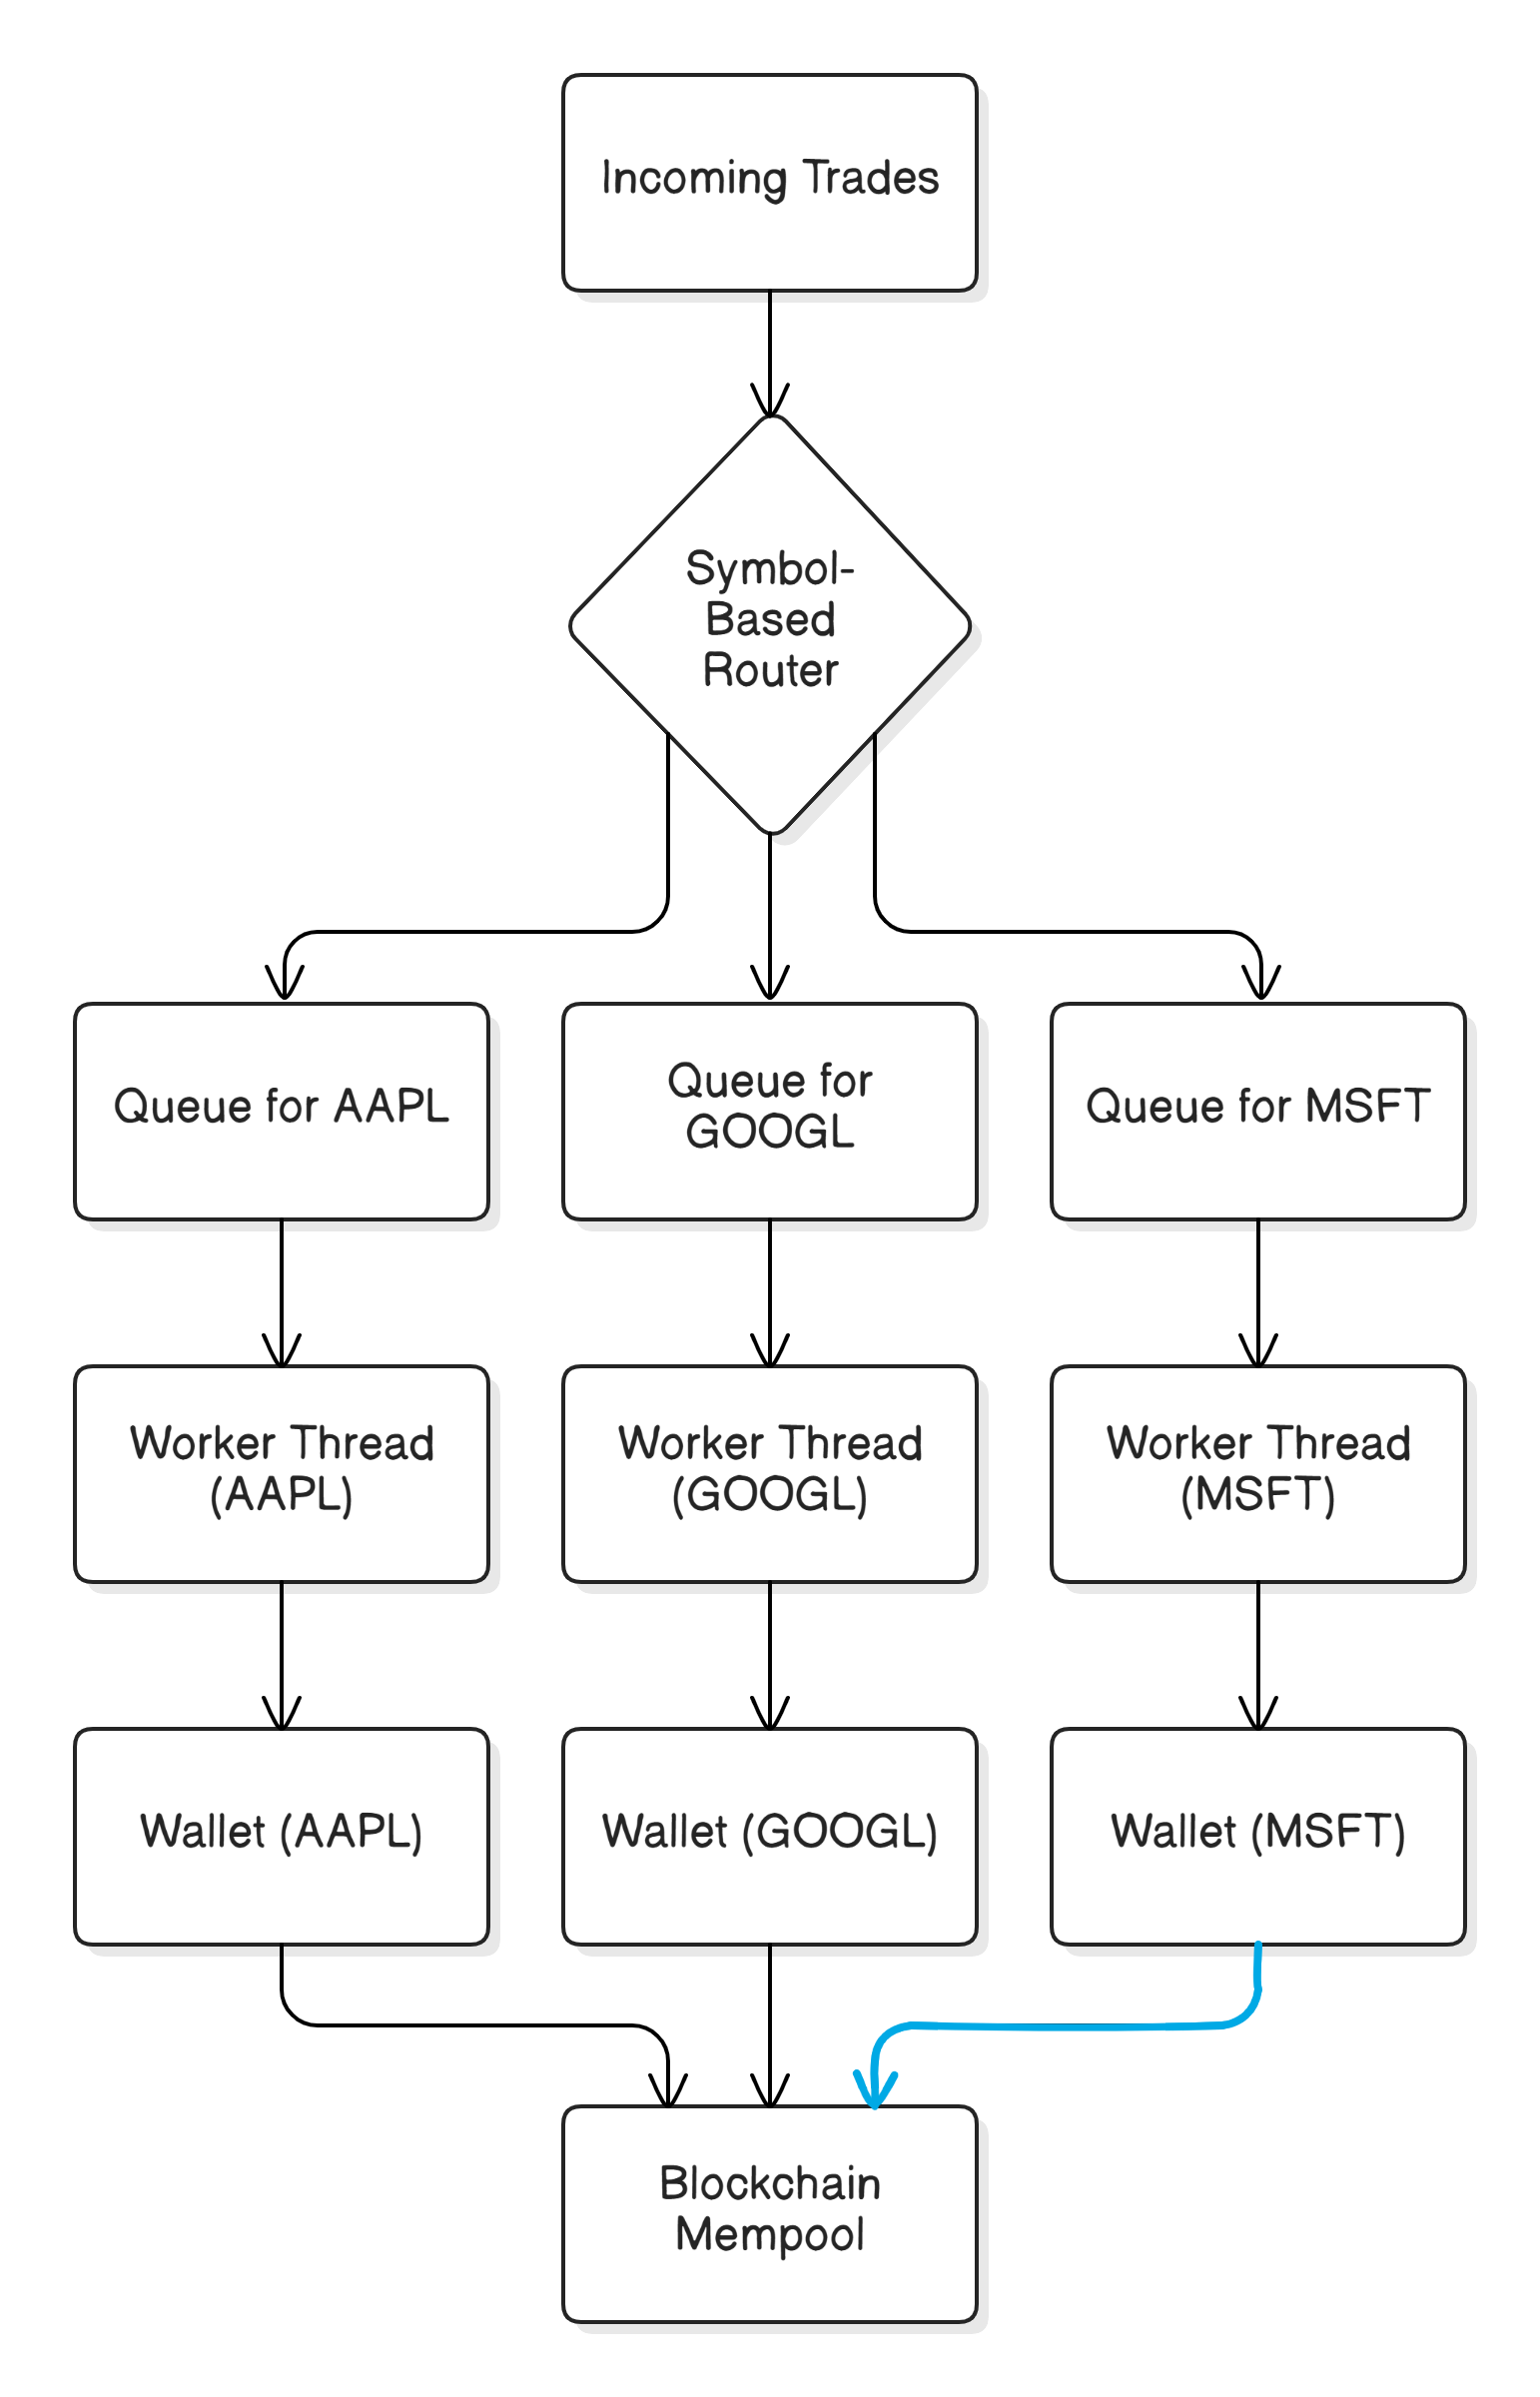
\includegraphics[width=0.82\linewidth]{images/symbol-sharded-lock-free-model.png}\\[0.1cm]
    \footnotesize\textbf{Fig.~5:} Symbol-sharded, lock-free design.
  \end{center}
  Trades are routed by symbol to independent queues and worker threads, each owning a dedicated wallet, removing cross-symbol lock contention entirely.
}

\block{Conclusions}{
  \begin{itemize}
    \setlength\itemsep{0.1em}
    \item A symbol-sharded, lock-free architecture achieves \textbf{31.19 tx/sec}, the highest throughput across all five studied variants.
    \item Naive concurrency fixes (multi-threading, multi-wallet) expose new bottlenecks rather than resolving throughput ceilings.$^{[2,4]}$
    \item Regulatory-compliant, high-throughput blockchain trading is achievable through careful \textbf{architectural co-design}, not brute-force parallelism.
    \item Future work: adaptive sharding and cross-chain generalisation.
  \end{itemize}
}

\block{Key References}{
  \small
  \begin{enumerate}
    \setlength\itemsep{0.05em}
    \item G.\ Wood, \textit{Ethereum: A Secure Decentralised Generalised Transaction Ledger} (Ethereum Yellow Paper), 2014.
    \item M.\ Moir, N.\ Shavit, ``Concurrent Data Structures,'' in \textit{Handbook of Data Structures and Applications}, D.\ P.\ Mehta, S.\ Sahni, Eds. Chapman \& Hall/CRC, 2004.
    \item T.\ L.\ Harris, ``A Pragmatic Implementation of Non-Blocking Linked-Lists,'' in \textit{Distributed Computing---DISC 2001}, LNCS vol.\ 2180. Springer, 2001, pp.\ 300--314.
    \item G.\ M.\ Amdahl, ``Validity of the Single Processor Approach to Achieving Large Scale Computing Capabilities,'' in \textit{Proc.\ AFIPS Spring Joint Computer Conference}, 1967, pp.\ 483--485.
    \item J.\ L.\ Hennessy, D.\ A.\ Patterson, \textit{Computer Architecture: A Quantitative Approach}, 6th ed., Morgan Kaufmann, 2017.
    \item M.\ Thompson, D.\ Farley, M.\ Barker, P.\ Gee, A.\ Stewart, \textit{LMAX Disruptor: High Performance Alternative to Bounded Queues for Exchanging Data Between Concurrent Threads}, May 2011.
  \end{enumerate}
}

\end{columns}

\end{document}
